\section{Pellicola} \label{sec:pellicola}
Le pellicole sono il cuore della fotografia analogica, sono il supporto su cui viene impressa la foto.

In origine le fotografie venivano catturate su lastre di metallo o vetro, cosparse di materiali fotosensibili. Con l'avanzare delle scoperte, sia in ambito fotografico che non, siamo arrivati alla pellicola di celluloide, così come la conosciamo noi oggi.

Le prime pellicole erano in bianco e nero, negli anni sono poi stati trovi dei modi, applicando dei filtri colorati, per avere pellicole a colori.

\subsection{Bianco e nero} \label{subsec:pellicolabw}
Non verrà data una descrizione precisa di come sono costruire le pellicole, se ne descriveranno gli elementi più importanti per capire, anche solo concettualmente, come funzionano.

Una pellicola è composta da diversi strati, ognuno con uno scopo ben preciso. Lo strato che più ci interessa è quello fotosensibile.

Lo strato fotosensibile è un'emulsione di cristalli di \textit{alogenuro d'argento} in un gel. I cristalli, che sono fotosensibili, se esposti alla luce diventano più scuri, in questo modo viene esposta la pellicola.

Notiamo che le zone di luce della foto, appaiono sulla pellicola come zone più scure, mentre le zone scure rimangono invariate e sono più chiare. Per questo le foto scattate con queste pellicole sono dette \textbf{negativi}.


\subsection{Colori} \label{subsec:pellicolacolori}
Le pellicole a colori funzionano in modo molto simile alle controparti in bianco e nero, con la differenza che tra i diversi strati della pellicola ce ne sono alcuni (in aggiunta a quelli già presenti) che filtrano la luce e fanno apparire i colori nella foto finale.


\subsection{ISO e grana} \label{subsec:isograna}
Caratteristica importante di tutte le fotocamere analogiche è che la sensibilità alla luce (i.e. ISO) è legata alla pellicola; non si può cambiare la sensibilità ad ogni scatto, così come si può fare con un sensore digitale, ma si può far solo ad ogni cambio pellicola.

Per indicare gli ISO di una pellicola si parla anche di \textit{velocità} della pellicola.

Come abbiamo visto, sui sensori (vedi \nameref{sec:sensore}), aumentare gli ISO comporta più rumore nella foto.
Le pellicole non generano rumore come i sensori, ma hanno quella che viene chiamata \textbf{grana}.

Sebbene rumore e grana sembrino simili, la grana è solitamente più piacevole all'occhio; l'effetto grana è anzi un effetto che piace ed è spesso ricercato.

Sono inoltre diversi i motivi per cui i sensori generano rumore e le pellicole la grana.

Il rumore nei sensori è introdotto da una moltitudine di eventi, quali la dimensione del sensore, fluttuazioni di voltaggio durante la conversione del segnale in digitale, temperature del sensore, e altri.

La grana delle pellicole invece è dovuta ai cristalli di alogenuro d'argento. Pellicole più sensibili (i.e. ISO più alti) hanno cristalli più grandi che producono una grana più grande.


\subsection{Pellicola ortocromatica} \label{subsec:pellicolaorto}
Le prime pellicole in bianco e nero erano ortocromatiche, ovvero non erano sensibili alla luce rossa.

La non-sensibilità è su una porzione dello spettro di luce visibile, possiamo semplificare dicendo semplicemente che il colore rosso non viene catturato da queste pellicole.

Tutto ciò è rosso quindi non viene impresso sulla pellicola, e nella foto finale rimane nero.
I corpi rossi in realtà difficilmente rimangono perfettamente neri, in una scena possono esserci molto riflessi di altri colori che rimbalzare sul rosso e vengono catturati dalla pellicola, in questo caso i colori che rimbalzano sul rosso vengono esposti, il corpo prende un po' di colore.

Nella Figura~\ref{fig:orto} una foto scattata con pellicola ortocromatica.

\begin{figure}[H]
    \centering
    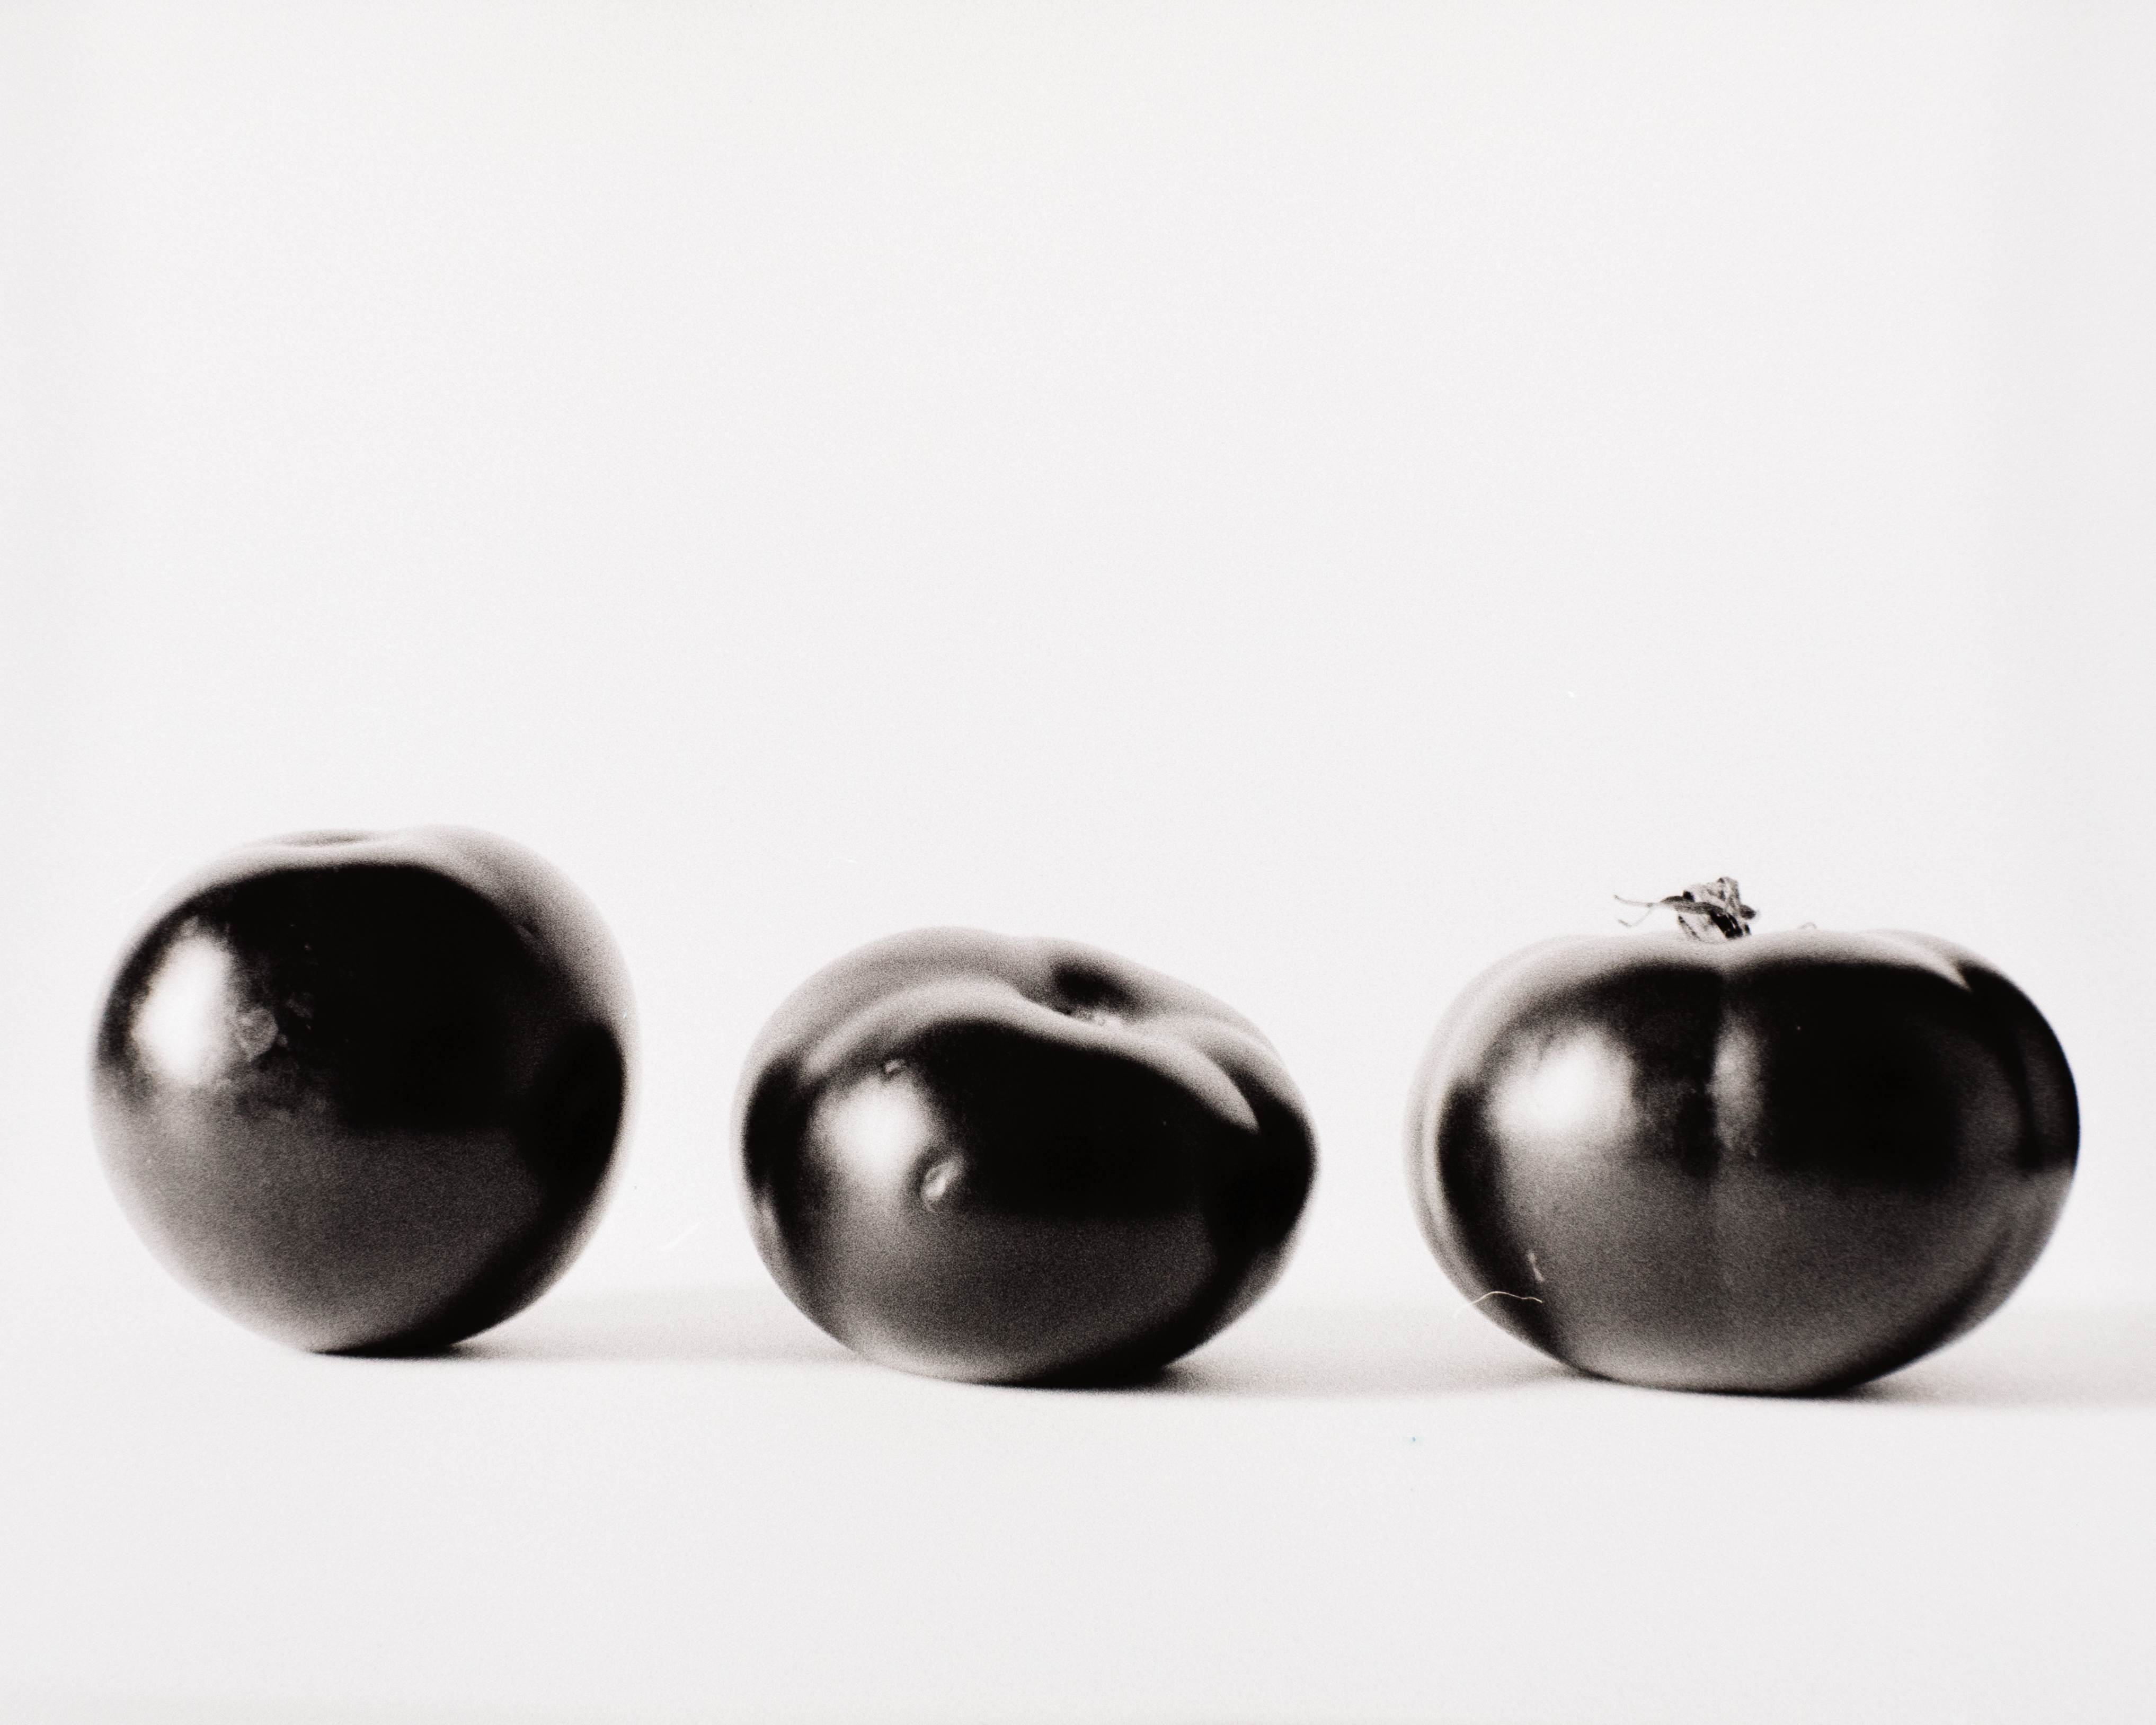
\includegraphics[width=\textwidth]{pomodori.jpg}
    \caption{
        Tre pomodori rossi fotografati con pellicola Rollei Ortho Plus 25. Si noti come la fonte di luce sulla sinistra (di colore bianco) rimbalzi e sia visibile sui pomodori, così come nella parte bassa dei pomodori è visibile il riflesso del foglio di carta bianco su cui sono appoggiati
    }
    \label{fig:orto}
\end{figure}

%Le pellicole ortocromatiche, grazie anche a tv e cinema, sono il motivo per cui ci immaginiamo le camere oscure per lo sviluppo delle pellicole illuminate con una lampadina rossa.
%Quando si sviluppa una pellicola bisogna lavorare nel buio più assoluto, un'infiltrazione di luce verrebbe catturata dalla pellicola e rovinerebbe le foto fatte.
%Se però la pellicola  non è sensibile al colore rosso, allora si può usare una luce rossa per illuminare un poco la stanza, così da poter lavorare molto più facilmente.
%
%Se però la pellicola è sensibile al colore rosso allora non si può usare una luce rossa nella camera oscura, altrimenti il rosso verrebbe di fatto cattura dalla pellicola e le foto a quel punto sarebbero perse per sempre.


\subsection{Pellicola pancromatica} \label{subsec:pellicolapan}
Pancromatico viene dal greco, e si può tradurre come \textit{tutti i colori}.

Le pellicole pancromatiche sono quelle sensibili a tutti i colori visibili, ovvero a tutte le lunghezze d'onda dello spettro visibile.


\subsection{Pellicola infrarossi} \label{subsec:pellicolair}
Esistono pellicole in bianco e nero che vanno oltre le pellicole pancromatiche, e non solo sono in grado di catturare tutto lo spettro di luce visibile, ma sono sensibili anche alle luci infrarossi.

Come appare una luce infrarossi su queste pellicole? Sono in bianco e nero, quindi un sorgente di luce infrarossa apparirà tanto più bianca quanto più intensa sarà.